% Write a piece of TikZ code to show the pedigree diagram of inbreeding between half cousins.
% Use solid circles with gradient fills to display nodes. Display the labels in the diagram where applicable.
% Use any of the required tikz packages to make the code less verbose.

\documentclass{article}
\usepackage{tikz}
\usetikzlibrary{trees,shapes,positioning,arrows.meta,shadows.blur}
\begin{document}

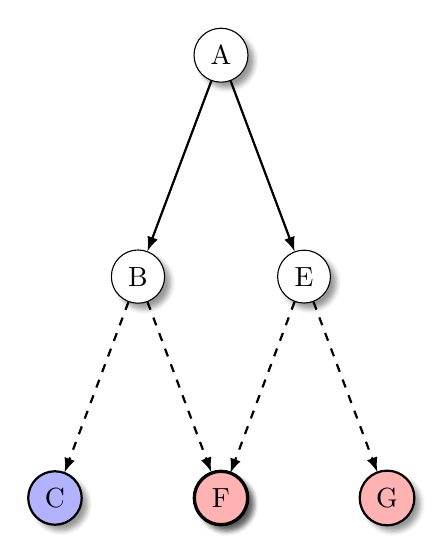
\begin{tikzpicture}[  sibling distance=6em,  level distance=8em,  every node/.style={draw,circle, fill=white, font=\fontsize{10}{10}\selectfont, text centered, blur shadow},  edge from parent/.style={draw,thick,-latex},  edge from parent path={(\tikzparentnode) -- (\tikzchildnode)}]

\node {A}
child { node {B} 
  child { node[fill=blue!30] {C} edge from parent[dashed] }
  child { node[fill=blue!30] {D} edge from parent[dashed] }
}
child { node {E} 
  child { node[fill=red!30] {F} edge from parent[dashed] }
  child { node[fill=red!30] {G} edge from parent[dashed] }
};
\end{tikzpicture}

\end{document}